
\begin{figure}[ht]
\centering
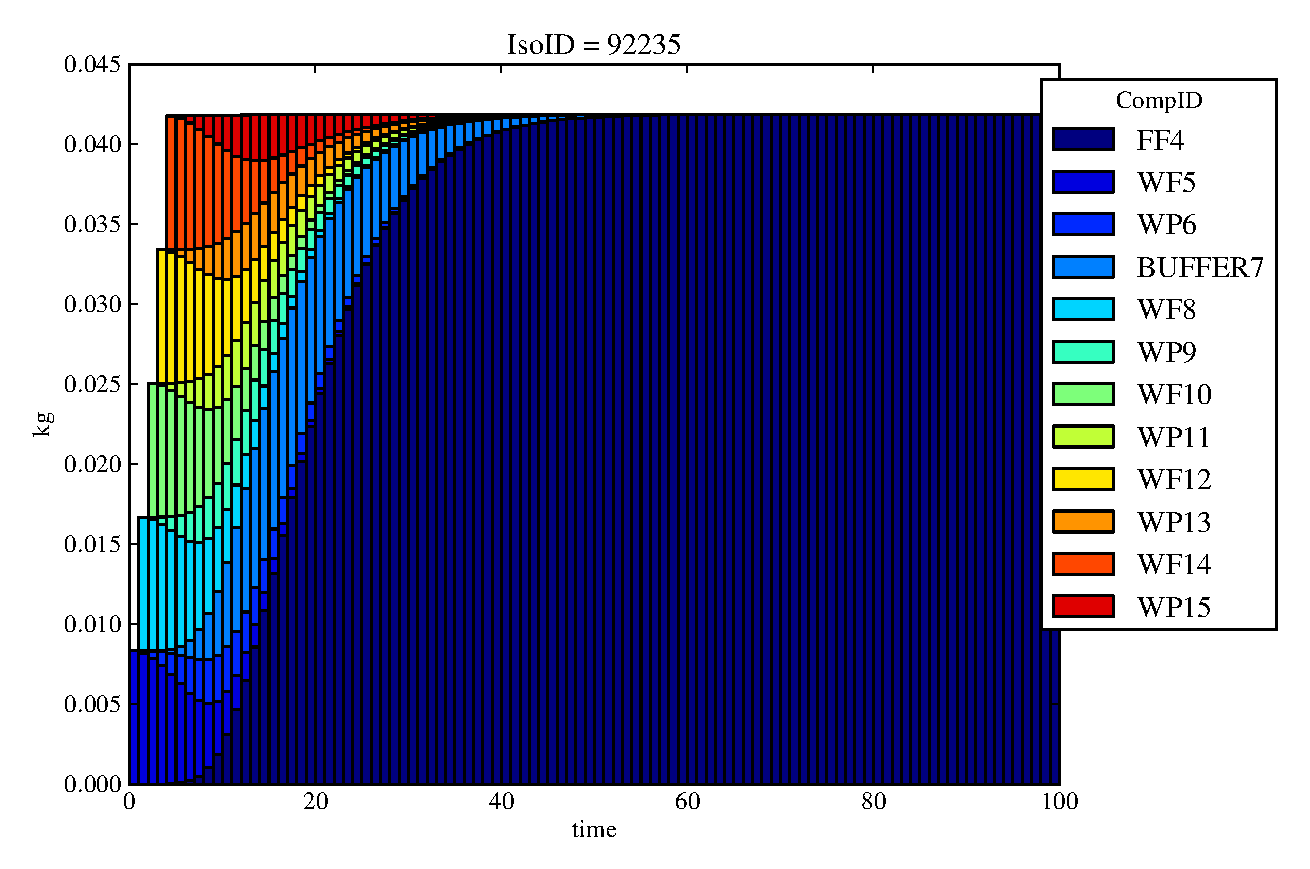
\includegraphics[width=0.6\textwidth]{./results/images/mcIII.eps}
\caption[$^{235}U$ residence. Mixed Cell Coupled Sorption and Solubility Limitation.]{
For the MCIII case in which containment is affected by solubility limitation,
        ($F_{d}=0.1$ for all components), $^{235}U$ travels through waste 
        packages (WPN), their corresponding waste forms (WFN), and the surrounding 
        buffer (BUFFER7) more slowly than in the MCI case
        before permanent residence in the far field component (FF).
}
\label{fig:mcIIIall}
\end{figure}

\begin{figure}[ht]
\centering
  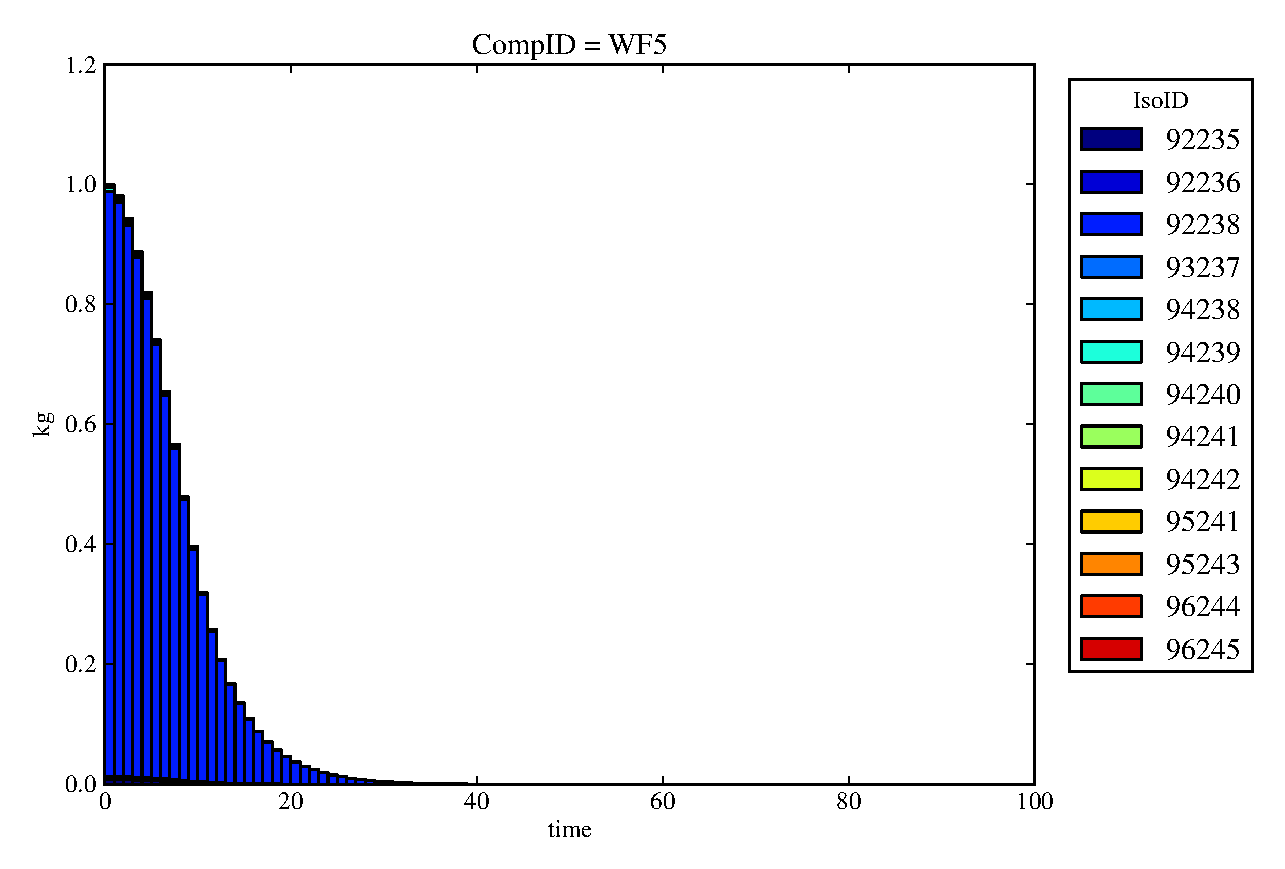
\includegraphics[width=0.6\textwidth]{./results/images/mcIII1.eps}
  \caption[Case MCIII Waste Form Contaminants.]{
    Waste Form 5 ($F_d = 0.1$, $S_{ref} = 0.001kg/m^3$) releases material with degradation.
    }
  \label{fig:mcIIIwf5}
\end{figure}


\begin{figure}[ht]
\centering
  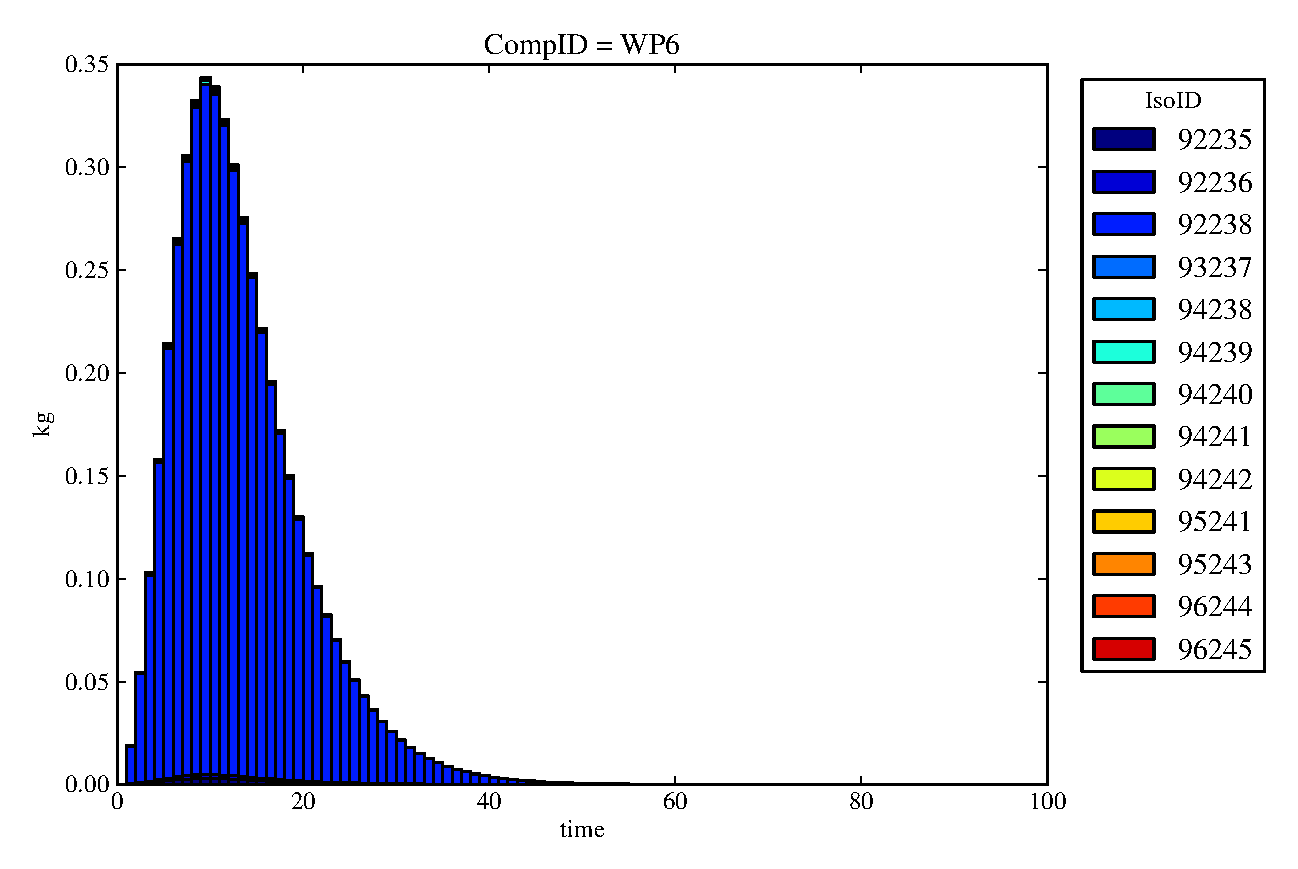
\includegraphics[width=0.6\textwidth]{./results/images/mcIII2.eps}
  \caption[Case MCIII Waste Package Contaminants.]{
    Waste Package 6 ($F_d = 0.1$, $S_{ref}=0.001kg/m^3$) receives then releases material.
    }
  \label{fig:mcIIIwp6}
\end{figure}

\begin{figure}[ht]
\centering
  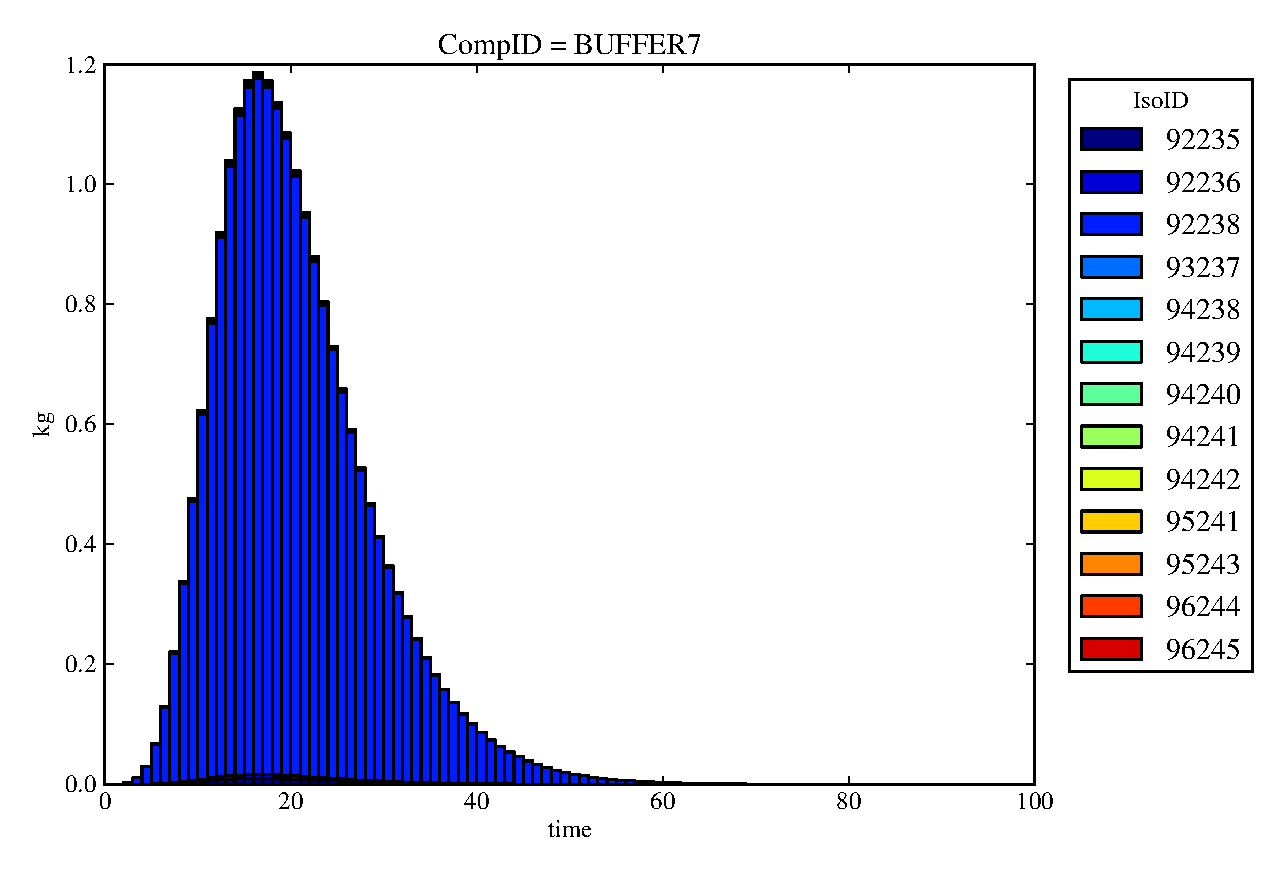
\includegraphics[width=0.6\textwidth]{./results/images/mcIII3.eps}
  \caption[Case MCIII Buffer Contaminants]{
    The Buffer, component 7 ($F_d=0.1$, $S_{ref}=0.001kg/m^3$), receives and then releases material.
    }
  \label{fig:mcIIIbuff}
\end{figure}

\begin{figure}[ht]
\centering
  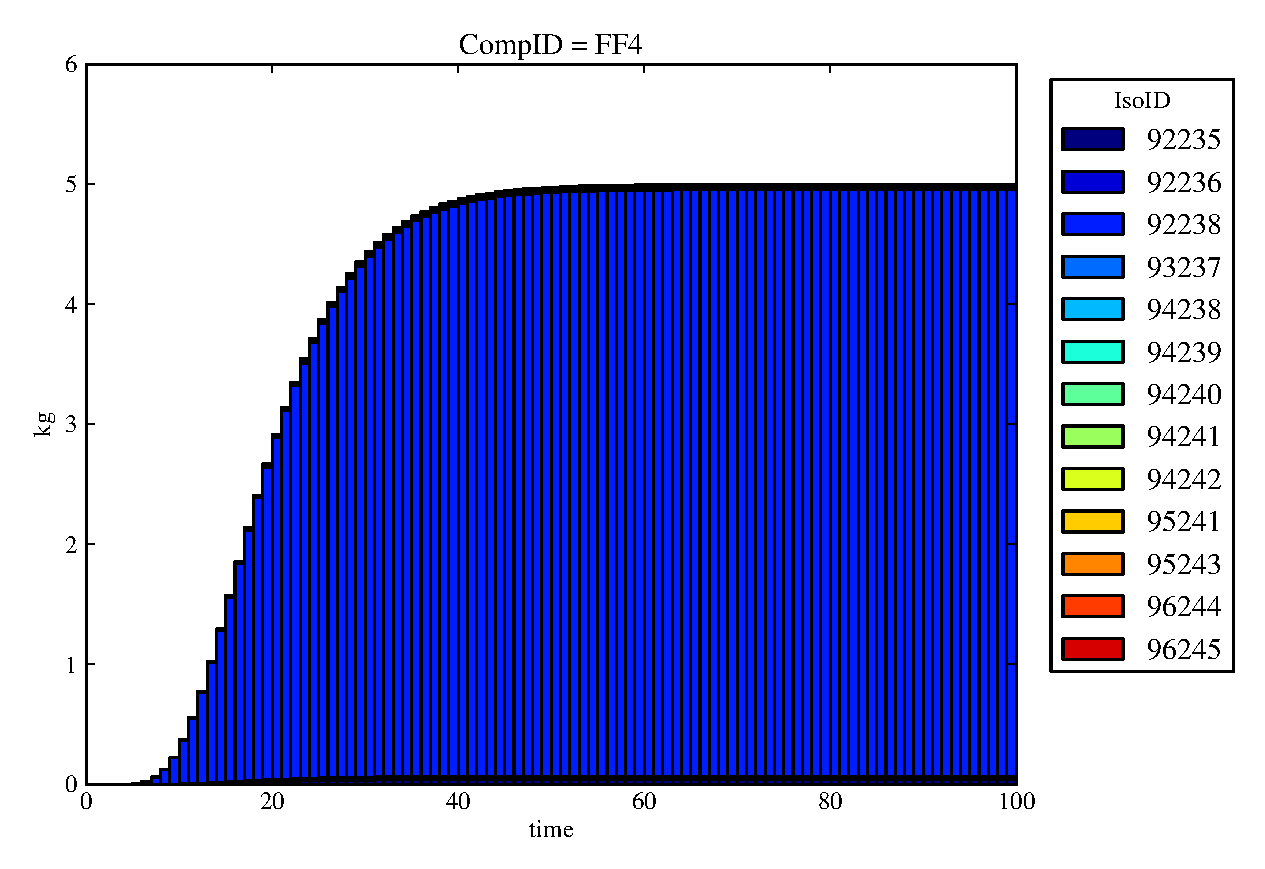
\includegraphics[width=0.6\textwidth]{./results/images/mcIII0.eps}
  \caption[Case MCIII Far Field Contaminants.]{All material is released into
    the Far Field, component 4 ($F_d=0.0$, $S_{ref} = 0.001kg/m^3$).}
  \label{fig:mcIII}
\end{figure}

